\documentclass{beamer}

\usepackage{tikz}
\usetikzlibrary{shapes,arrows}
\usepackage{biblatex}
\addbibresource{proposal.bib}

\setbeamertemplate{navigation symbols}{}
\usetheme{Montpellier}
\beamersetuncovermixins{\opaqueness<1>{25}}{\opaqueness<2->{15}}

\begin{document}
\title{Bayesian parameter synthesis of Markov population models.}
\author{Nhat-Huy Phung}

\begin{frame}
  \titlepage
\end{frame}

\begin{frame}
  \frametitle{Table of contents}
  \tableofcontents
\end{frame}

\section{Motivation}
\begin{frame}
  \frametitle{Motivation}
  In this thesis, we study \textit{population processes}. Kingman
  \cite{10.2307/3212273} defines \textit{population
    processes} as stochastic models of discrete state spaces, in which:
  \begin{itemize}
    \item Each state in the state space represent the number of individuals in a
          category or a colony.
    \item Changing from a state to another state represents an increase or
          decrease of the number of individuals.
  \end{itemize}
\end{frame}

\begin{frame}
  \frametitle{Example}
  Examples of population process:
  \begin{itemize}
    \item A bee colony of initially $n$ individuals. Assume that one bee can sting
          randomly with a probability $p$, we can construct a parametric Discrete
          Time Markov Chain to represents the population process.
    \item Number of computation nodes which are alive in a server cluster, with an
          assumption that an arbitrary node dies with probability $p$.
  \end{itemize}
  \begin{figure}[t]
    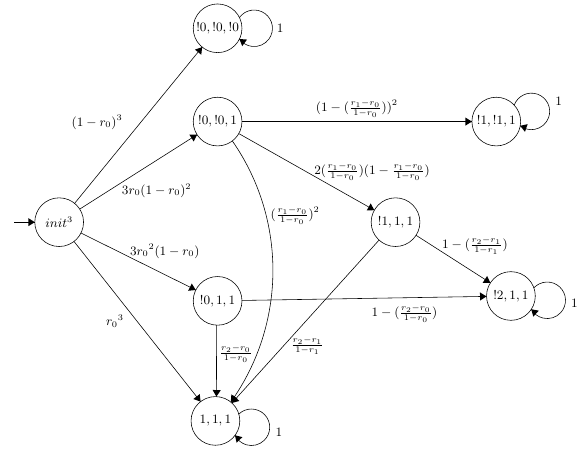
\includegraphics[height=0.5\textheight]{3bees.png} \centering
    \caption{A Markov population model of 3 bees (developed by Matej Hajnal and
      Tatjana Petrov)}
  \end{figure}
\end{frame}

\begin{frame}
  \frametitle{Question}
  As we study a Markov population process, the following questions are raised:
  \begin{itemize}
    \item \textit{Parametric model}: How can we encompass unknown features into
          the population model?
    \item \textit{Parameter synthesis}: Given a parametric population model and
          observed data of the population, how can we infer the model parameters?
    \item \textit{Model composition}: How can we generalize aggregate a
          multi-agents population model from single-agent behaviour model?
  \end{itemize}
  In the scope of this thesis, we limit our study to discrete-time model.
\end{frame}

\begin{frame}
  \frametitle{Approach}
  \begin{itemize}
    \item Model individual behaviour after a parametric Markov Decision Process.
    \item Model collective behaviour by compositing individual models to a
          parametric Discrete Time Markov Chain.
    \item Use data-informed Bayesian inference to synthesize the parametric
          Discrete Time Markov Chain parameters.
  \end{itemize}
\end{frame}

\section{Data}
\begin{frame}
  \frametitle{Data}
  As we use Bayesian inference, we need data.
  \begin{itemize}
    \item In the thesis, we use synthetic data, obtained by simulating the
          parametric model using a concrete assignment of parameters.
    \item Using \textit{synthetic data} has an advantage over using real data.
          As the concrete parameters are known, it is possible to measure the
          distance between the synthesized parameters and true parameters.
  \end{itemize}
\end{frame}

\section{Model and properties}
\begin{frame}
  \frametitle{Single agent model.}
  We model the behaviour of a single bee as a Markov Decision Process. Let
  $\mathcal{S}$ be the individual model, we have
  \begin{align*}
    \mathcal{S} = (S, A, P_a, R_a)
  \end{align*}
  in which
  \begin{itemize}
    \item $S$ is the set of states.
    \item $A$ is the set of actions.
    \item $P_a(s,s')$ is the probability of transitioning from state $s$ to state
          $s'$ given action $a$.
    \item $R_a(s,s')$ is the \textit{reward} received after transitioning from
          state $s$ to state $s'$ given action $a$.
  \end{itemize}
\end{frame}

\begin{frame}
  \frametitle{Single agent model.}
  Example of a single bee model
  \begin{figure}[t]
    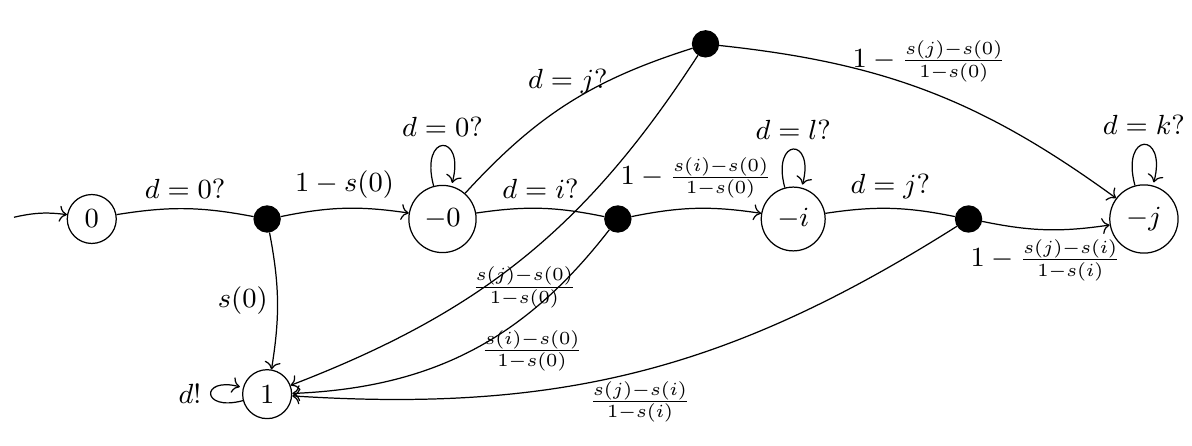
\includegraphics[height=0.4\textheight]{smodel.png} \centering
    \caption{Generic single bee model (developed by Matej Hajnal and
      Tatjana Petrov)}
  \end{figure}
\end{frame}


\begin{frame}
  \frametitle{Multi-agent model}
  To model collective behavior of multiple agents, we construct product of
  individual models. Let $\mathcal{M}$ be the multiple agents pDTMC model, we constr
  \begin{align*}
    \mathcal{M} = (\mathcal{S}_1||\mathcal{S}_2||\ldots||\mathcal{S}_k)
  \end{align*}
  Composition of MDP are mentioned in \cite{sokolova2004probabilistic}.
  Asynchronous and synchronous semantics for constructing pDTMC from multiple
  pMDP are currently developed by Tatjana Petrov.
\end{frame}

\begin{frame}
  \frametitle{Multi-agent model}
  Example of a multi-agent model.
  \begin{figure}[t]
    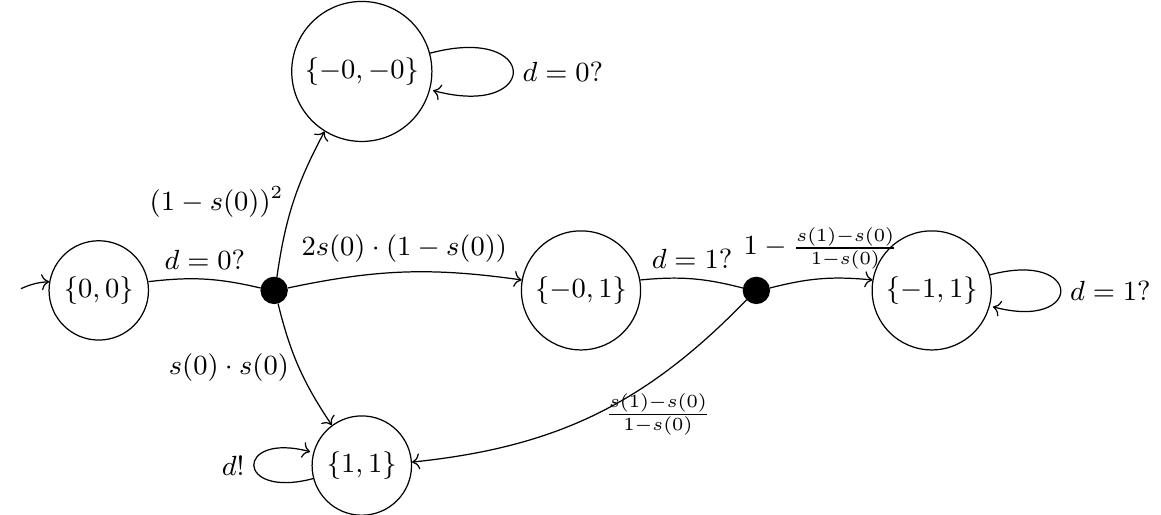
\includegraphics[height=0.4\textheight]{mmodel.png} \centering
    \caption{Example of 2 bees model (developed by Matej Hajnal and
      Tatjana Petrov)}
  \end{figure}
\end{frame}

\begin{frame}
  \frametitle{Properties}
  \textbf{Question:} How can different parameters of single agent affect the
  population?\\
  \textbf{Answer:}
  Given a model $\mathcal{M}_\Theta$, to find the probability of having a
  certain number of individuals at the steady state, we
  \begin{itemize}
    \item represents population at steady state by a BSCC $s_i$, with $i$ is the
          population size.
    \item checking the model of against $PCTL P_{?} (FG s_i)$
  \end{itemize}

  We can survey further constraints on model and properties:
  \begin{itemize}
    \item Surviving percentage: lumping BSCCs.
    \item Reduce parameter space: apply a linear/sigmoidal constraints over
          parameter space $\Theta$.
  \end{itemize}

\end{frame}


\section{Framework}
\begin{frame}
  \frametitle{Related work}
  Gareth Molyneux et al. \cite{molyneux2019bayesian} presented \textit{ABCSeq} framework
  for Bayesian Verification of CTMC.
  \begin{figure}[t]
    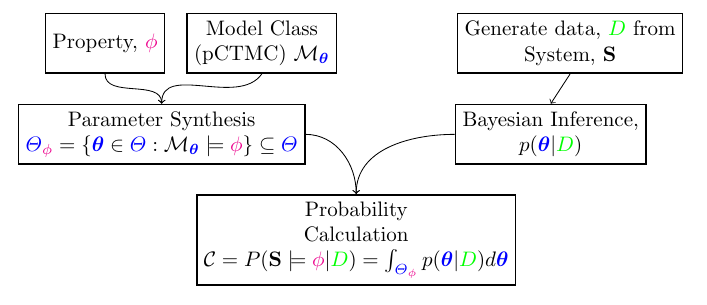
\includegraphics[height=0.5\textheight]{molyneux2019.png} \centering
    \caption{ABCSeq Bayesian verification framework.}
  \end{figure}
\end{frame}

\begin{frame}
  \frametitle{Related work}
  In \cite{molyneux2020abc}, the authors present \textit{ABC(SMC)2} to
  improve \textit{ABCSeq} framework for better performance.
  \begin{figure}[t]
    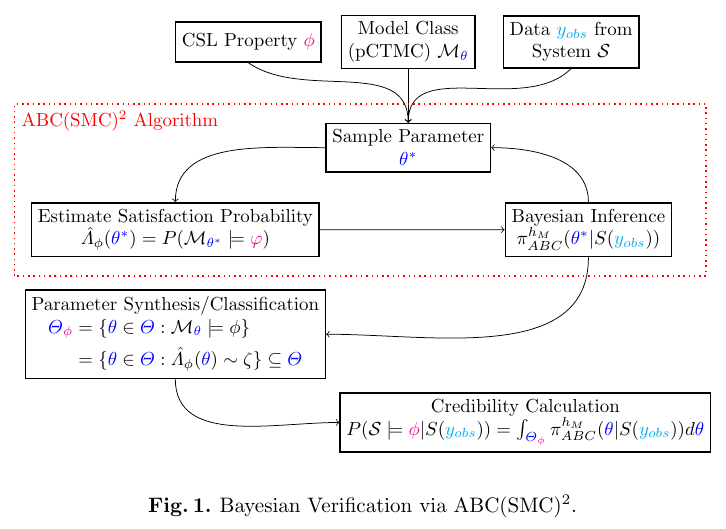
\includegraphics[height=0.7\textheight]{molyneux2020.png} \centering
  \end{figure}
\end{frame}

\begin{frame}
  \frametitle{Proposed Framework}
  We develop a similar framework for parameter synthesis of pDTMC based on
  \cite{molyneux2020abc} and \cite{molyneux2019bayesian}. Compare to the work by
  Gareth Molyneux et al., our framework should
  \begin{itemize}
    \item Works with discrete time model.
    \item Verify PCTL property.
    \item Since the model is of discrete-time, the closed form solution (symbolic)
          for a PCTL property is in some cases obtainable. In such cases, we can
          compute the exact likelihood without simulation.
  \end{itemize}
\end{frame}

\begin{frame}
  \frametitle{Proposed Framework}
  \begin{figure}[t]
    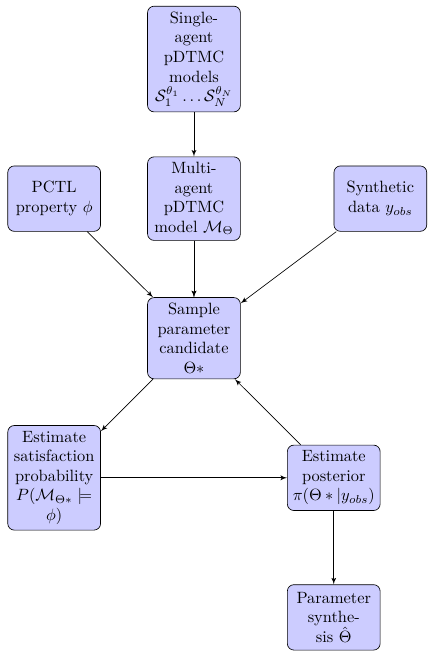
\includegraphics[height=\textheight]{framework.png} \centering
  \end{figure}
\end{frame}

\begin{frame}
  \frametitle{Tools}
  For probabilistic model checking and parameter synthesis, we use STORM
  probabilisttic model checker
  \begin{itemize}
    \item \textbf{Extensible}: High quality C++ APIs <- this is important.
    \item \textbf{Scalable}: Faster compare to PRISM.
    \item \textbf{Capable}: STORM factorizes symbolic results on-the-fly.
  \end{itemize}
\end{frame}

\section{Case study}
\begin{frame}
  \frametitle{Case study}
  We study the defensive behaviour of a bee colony.
  \begin{itemize}
    \item Bees response to stimulations from the environment by \textit{stinging}.
    \item After \textit{stinging}, an individual bee releases \textit{pheromone}
          and dies.
  \end{itemize}
  Our questions concerns the relation between the concentration of pheromone in
  the environment and the aggressiveness of each individual in the colony.
\end{frame}

\begin{frame}
  \frametitle{Case study}
  As we study the biological system, we have the following research questions:
  \begin{enumerate}
    \item Given a population of bee, how many individuals left in the steady
          state.
    \item How does an individual's behaviour change the collective behaviour? Does
          each individual become more aggresive given the
  \end{enumerate}
\end{frame}

\section{Timeline}
\begin{frame}
  \frametitle{Timeline}
  Thesis milestones
  \begin{enumerate}
    \item \textbf{07.12.2020}: Model and properties lists.
    \item \textbf{21.12.2020}: Framework implementation and results.
    \item \textbf{10.01.2021}: Model improvement.
    \item \textbf{30.01.2021}: Thesis submission.
  \end{enumerate}
  Progress is reported weekly.
\end{frame}

\section{References}
\begin{frame}
  \frametitle{References}
  \printbibliography
\end{frame}

\end{document}